\documentclass{beamer}

\mode<presentation> {\usetheme{Szeged}}
%Dresden, Berlin, Ilmenau, Szeged are my favorites

\usepackage[english]{babel}
\usepackage{graphicx} % Allows including images
\usepackage{booktabs} % Allows the use of \toprule, \midrule and \bottomrule in tables
\usepackage{subcaption}
\usepackage{xcolor}
\usepackage{tcolorbox}
\usepackage{tabularx}
\usepackage{textcomp}
\usepackage{comment}
\usepackage{amsmath}
\usepackage[version=4]{mhchem}
\usepackage{fixltx2e}
\usepackage{MnSymbol,wasysym}
\captionsetup[figure]{labelformat=empty}
\usepackage{hyperref}
\usepackage{verbatim}

\usepackage{allrunes} 
\usepackage[safe]{tipa} % for superscribed letters using \sups{}{}
\renewcommand{\sups}[2]{\textipa{\tipaUpperaccent[.2ex]{%
 			\lower.8ex\hbox{\super{#2}}}{#1}}} % redefines appearance of superscribed letter
\usepackage[icelandic]{babel} 
\usepackage[T1]{fontenc} % specifies font encoding; T1 includes accented characters as individual glyphs, summing up to 256 characters (as opposed to the default font encoding (OT1) of TeX, which is 7-bit and uses fonts that have 128 glyphs)
\usepackage[utf8]{inputenc} % for UTF 8 support
\usepackage{yfonts} % includes gothic, fraktur and schwabacher font

\hypersetup{
colorlinks=true,
citecolor=violet,
linkcolor=black,   
urlcolor=blue}



\setbeamerfont{page number in head/foot}{size=\tiny}
\setbeamertemplate{footline}[frame number]

\title[LaTeX crash course]{\LaTeX \hspace{0.2mm} Crash Course \\
GRACE Transferable Skills
} % The short title appears at the bottom of every slide, the full title is only on the title page

\author{\href{mailto:antheajeanne.alberto@unibas.ch}{Dr.\ Anthea Alberto} \and \href{mailto:ina.serif@unibas.ch}{Dr.\ Ina Serif}}

\date{\centering \textbf{23.05.2023}\\
09:00-13:00}


\begin{document}

\begin{frame}
\titlepage % Print the title page as the first slide
\end{frame}


\begin{frame}{Intro}
\LARGE \centering Welcome back! 
\end{frame}

\begin{frame}{Agenda - 23.05.2023}
\begin{tabular}{ll}
09:00-10:15 & Images, tables, formulas\\
10:15-10:45 & Break\\
10:45-11:15 & Exercise\\
11:15-11:30 & Discussing the exercise\\
11:30-12:15 & Bibliographies\\
12:15-13:00 & Specialist packages, self-help competencies
\end{tabular} 
\end{frame}

%-------------
\section{Images, tables, formulas}
%------------

\begin{frame}{Images}
You begin by uploading your figure/graph/image to Overleaf's file menu on the left.\\~\\
This works either by clicking the dedicated button or via drag and drop.\\~\\
For other editors, it's advisable to have everything in the same folder, but it's also possible to use file paths.
\end{frame}

\begin{frame}{Images}
\begin{figure}
    \centering
    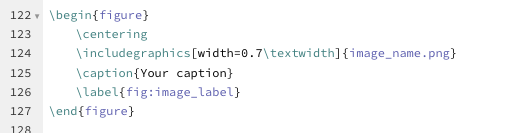
\includegraphics[width=0.7\textwidth]{figure_setup.png}
    \caption{The classic figure setup}
    \label{fig:fig_inception}
\end{figure}    
\end{frame}

\begin{frame}[fragile]{Images}
The classic \verb|\begin{figure}| consists of:\\
\vspace{1.5mm}
\begin{itemize}
    \item \verb|\includegraphics{}|: the name of the image you want to display
    \item \verb|\caption{}|: For captioning the image
    \item \verb|\label{}|: Label for cross-referencing; can also be added to sections, tables etc.
    \item \textit{caption} and \textit{label} are optional, but helpful
\end{itemize}    
\end{frame}

\begin{frame}[fragile]{Adjusting figure size}
Adjusting figure size:\\    
\begin{itemize}
    \item Often, the original size of a figure won't work for the document
    \item With the \textit{graphicx} package, you can easily adjust the size
    \item To adjust the size, use square brackets in the \verb|\includegraphics{}| command
\end{itemize}
\end{frame}

\begin{frame}{Adjusting figure size}
\begin{figure}
    \centering
    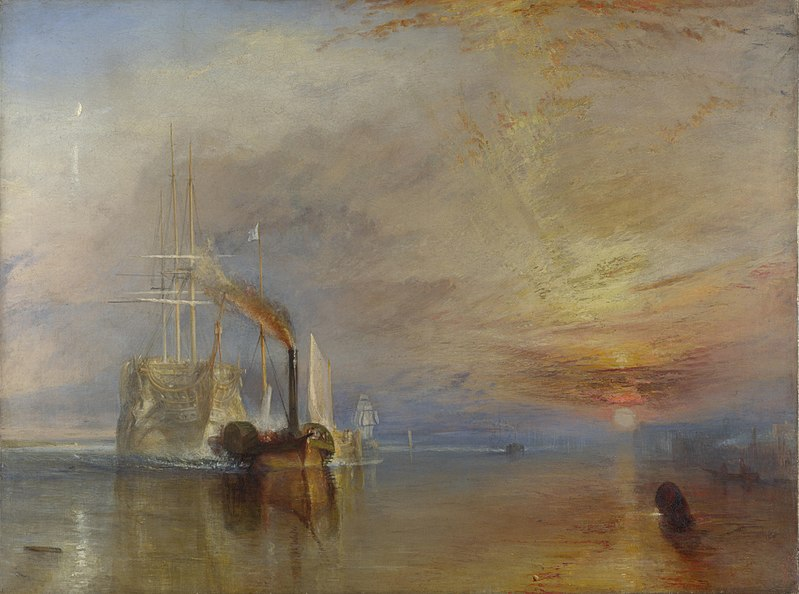
\includegraphics[width=0.7\textwidth]{temeraire.jpg}
    \caption{\textit{The Fighting Temeraire}, by JMW Turner (Source: \href{https://commons.wikimedia.org/wiki/File:The_Fighting_Temeraire,_JMW_Turner,_National_Gallery.jpg}{Wikimedia Commons})}
    \label{fig:temeraire_normal}
\end{figure}    
\end{frame}

\begin{frame}[fragile]{Adjusting figure size}
In the preceding slide, I used \verb|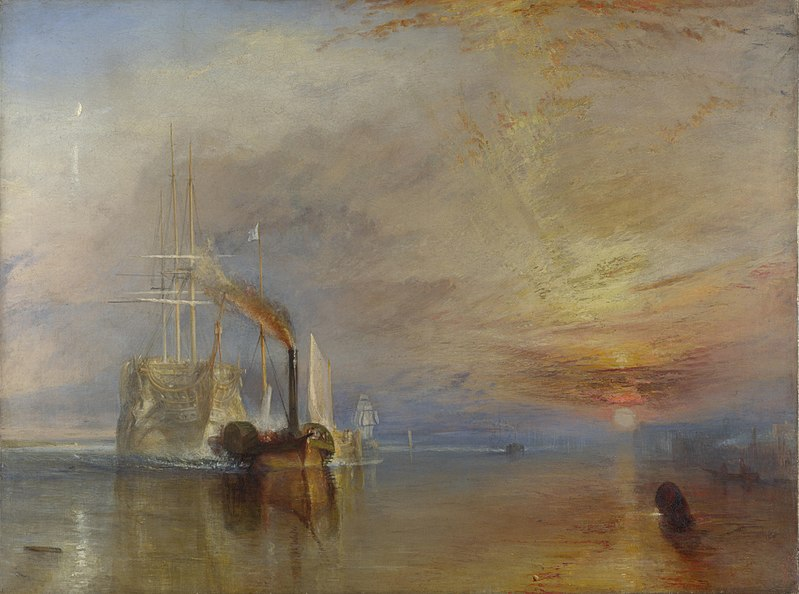
\includegraphics[width=0.7\textwidth]{temeraire.jpg}| to fit it neatly onto the slide.\\~\\
\textit{textwidth} here denotes the general area of text, and \verb|[width=0.7\textwidth]| means the image is scaled down to 70\% of textwidth.\\~\\
Another option is to use \textit{scale}, e.g. \verb|[scale=0.5]| to scale a figure down to 50\% of its size. 
\end{frame}

\begin{frame}{Adjusting figure size}
\begin{figure}
    \centering
    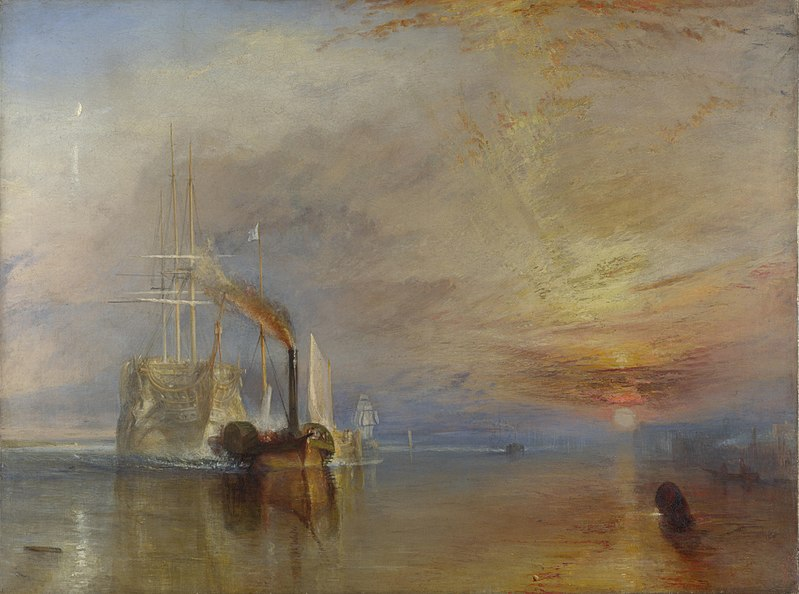
\includegraphics[scale=0.1]{temeraire.jpg}
    \caption{}
    \label{fig:temeraire_scale}
\end{figure} 
The picture is rather big, so scaling it down to 10\% (scale=0.1) of its original size will look like this.\\
See \href{https://www.overleaf.com/learn/latex/Questions/How_do_I_specify_the_size_of_an_image_in_LaTeX\%3F}{here} for a short tutorial.
\end{frame}

\begin{frame}[fragile]{Multiple images in one figure}
For putting multiple images in one figure, use the \textit{subfigure} environment.\\
\begin{figure}
    \centering
    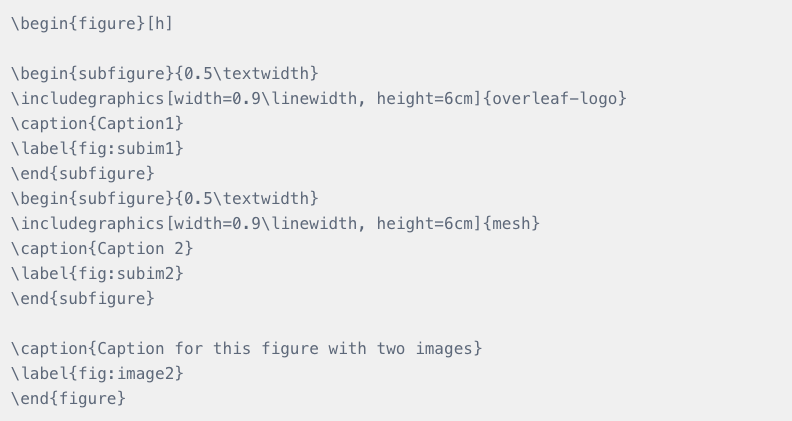
\includegraphics[width=0.8\textwidth]{subfigure.png}
    \caption{Example taken from the \href{https://www.overleaf.com/learn/latex/Positioning_images_and_tables\#Multiple_images_in_one_figure}{Overleaf tutorial}}
    \label{fig:subfigure}
\end{figure}
    
\end{frame}

\begin{frame}{Tables}
Creating tables in LaTeX follows a specific formula, but there are many costumisation options.\\
\begin{figure}
    \centering
    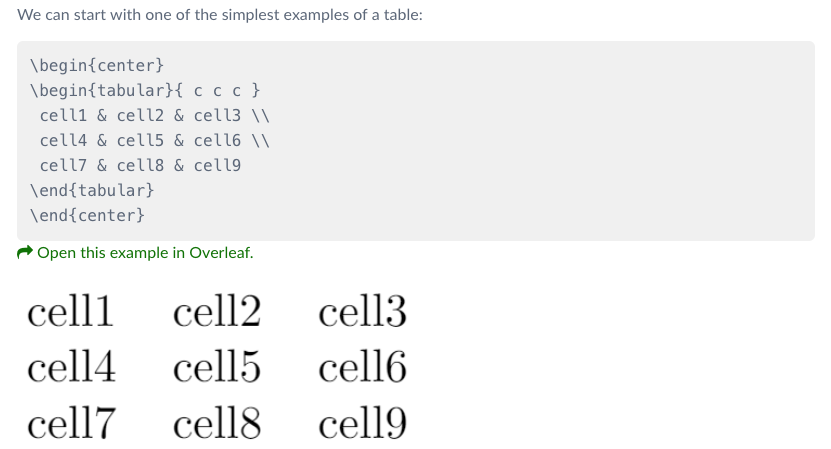
\includegraphics[width=0.8\textwidth]{table_simple.png}
    \caption{From the \href{https://www.overleaf.com/learn/latex/Tables}{Overleaf tutorial}}
    \label{fig:table_simple}
\end{figure}
\end{frame}

\begin{frame}[fragile]{Table components}
\verb|\begin{tabular}{ c c c }| is the beginning of the tabular environment and \verb|{ c c c }| indicates that I am building a table with three columns.\\ 
The elements within each cell are to be \textbf{c}entered (\textbf{l} and \textbf{r} are also options).\\~\\
The elements of each row are separated by a \&, and you need to put \verb|\\| at the end to skip to the next row, if it exists.\\
You can add as many rows as you like.
\end{frame}

\begin{frame}[fragile]{Tables}
If you want the columns separated by vertical lines, you can specify it by adding $\vert$ in between the c's:\\
\begin{figure}
    \centering
    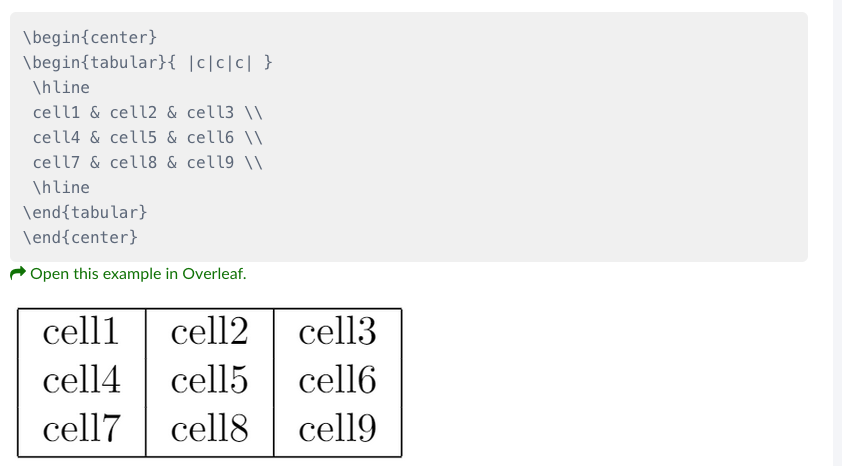
\includegraphics[width=0.75\textwidth]{tab_vert_bar.png}
    \caption{From the \href{https://www.overleaf.com/learn/latex/Tables}{Overleaf tutorial}}
    \label{fig:table_vertical}
\end{figure}
\end{frame}

\begin{frame}[fragile]{Tables}
For horizontal lines, just insert \verb|\hline| in between rows. You can add as many of them as you want.\\
\begin{center}
\begin{tabular}{||c c c c||} 
 \hline
 Col1 & Col2 & Col2 & Col3 \\ [0.5ex] 
 \hline\hline
 1 & 6 & 87837 & 787 \\ 
 \hline
 2 & 7 & 78 & 5415 \\
 \hline
 3 & 545 & 778 & 7507 \\
 \hline
 4 & 545 & 18744 & 7560 \\
 \hline
 5 & 88 & 788 & 6344 \\ [1ex] 
 \hline
\end{tabular}
\end{center}    
\end{frame}

\begin{frame}{Tables}
The code for the table on the previous slide looks like this:\\
\begin{figure}
    \centering
    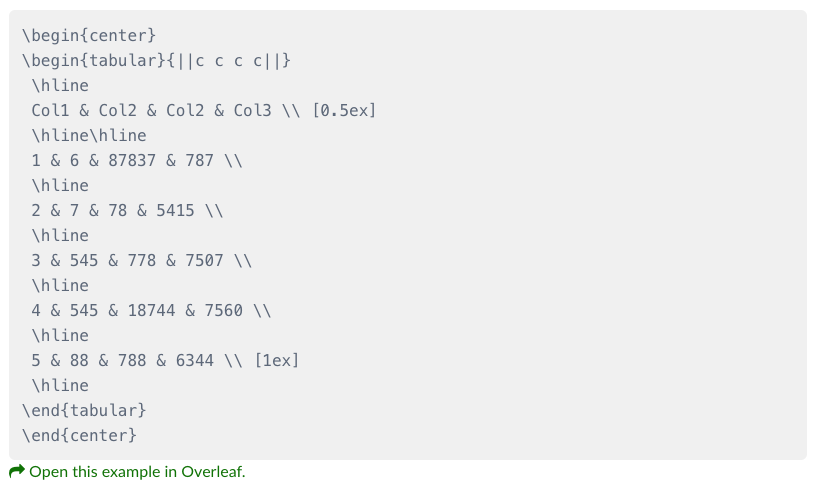
\includegraphics[width=0.75\textwidth]{table_complex.png}
    \caption{From the \href{https://www.overleaf.com/learn/latex/Tables}{Overleaf tutorial}}
    \label{fig:table_complex}
\end{figure}
\end{frame}

\begin{frame}{Table generator}
For quickly getting the basic syntax for a table, I recommend the \href{https://www.tablesgenerator.com/\#}{Table Generator} (or ChatGPT).\\
\begin{figure}
    \centering
    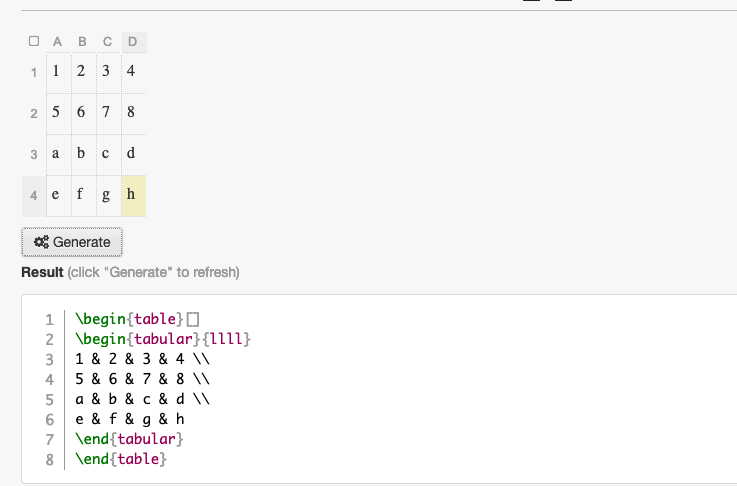
\includegraphics[width=0.6\textwidth]{table_generator.png}
    \caption{You can change and add to the template at will}
    \label{fig:table_generator}
\end{figure}
\end{frame}

\begin{frame}[fragile]{Placement}
There is a range of parameters that will determine a table's (or figure's) placement. First, you wrap the \textit{tabular} environment into a more generic \textit{table} environment.\\~\\
\pause
After \verb|\begin{table}|, put \verb|[h!]| (\textit{h} stands for \textit{here}) if you want to put the table exactly where it appears in the editor (i.e., exactly after one specific paragraph).\\~\\
\pause
The ! overrides internal LaTeX parameters. Simply putting \verb|[h]| would merely put the table \textit{here, approximately}. 
\end{frame}

\begin{frame}{Placement options}
\begin{itemize}
    \item \textbf{h} : place table or figure \textit{here}, approximately
    \item \textbf{t} : place table or figure at \textit{top} of the page
    \item \textbf{b} : place table or figure at \textit{bottom} of the page
    \item \textbf{p} : place table on special \textit{page}
    \item \textbf{!} : override internal LaTeX parameters
    \item \textbf{H} : roughly equal to h!; from the \textit{float} package
    \item You can put multiple options and only exclude those you definitely do not want 
\end{itemize}    
\end{frame}

\begin{frame}{Tables}
If you use a statistical software like R, there is likely a package or add-on that will create LaTeX versions of tables, e.g. of regressions.\\~\\
You can copy them into your document and adjust them as needed.\\~\\
An example for R is the \href{https://cran.r-project.org/web/packages/stargazer/stargazer.pdf}{stargazer} package.
\end{frame}

\begin{frame}{Tables}
\begin{figure}
    \centering
    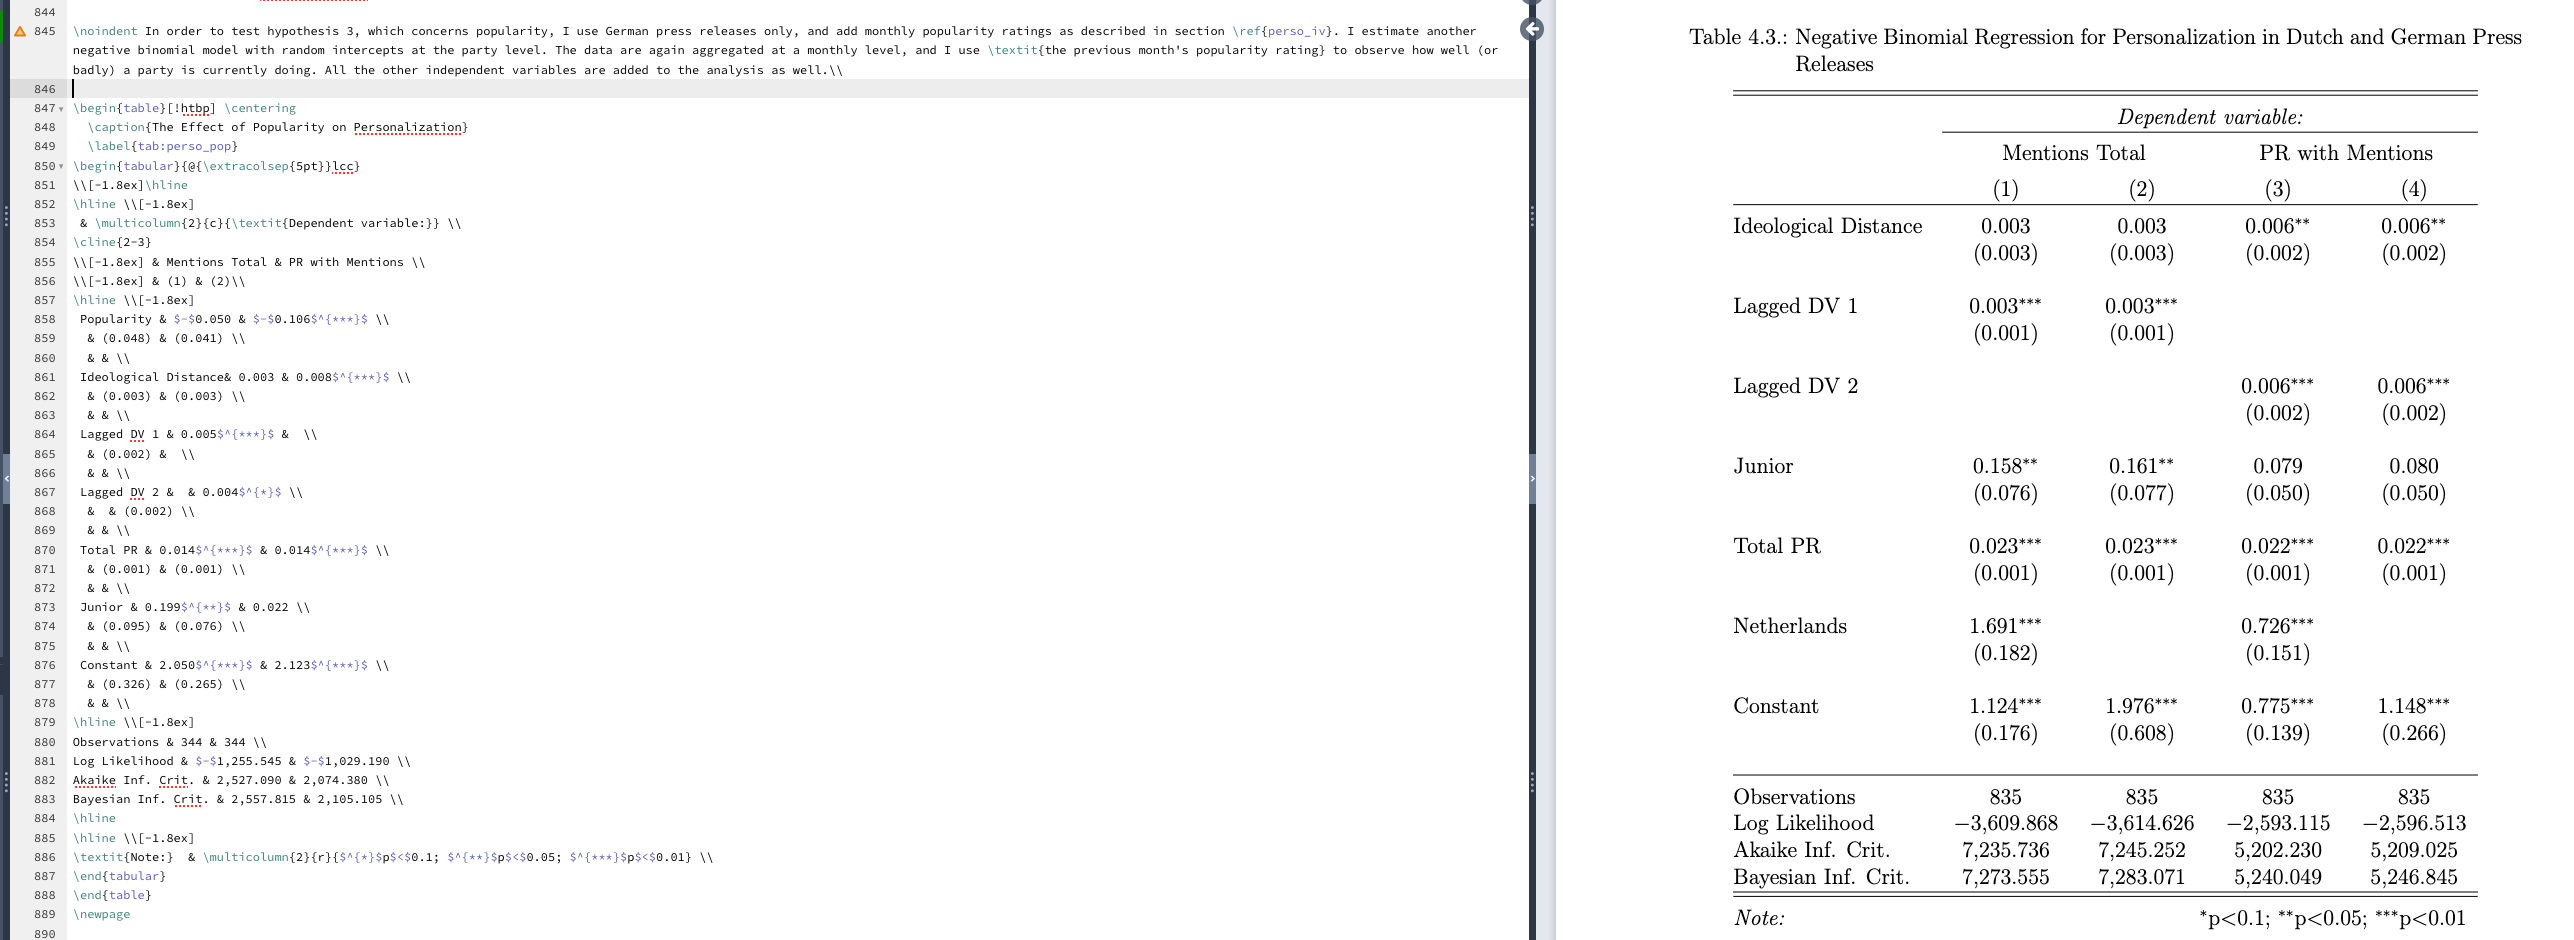
\includegraphics[width=\textwidth]{stargazer.png}
\end{figure}    
\end{frame}

\begin{frame}[fragile]{Formulas}
Inline formulas and equations are written using \$ on each side.\\~\\
E.g. $f(x) = x^2$ looks like this in an editor: \verb|$f(x) = x^2$|\\~\\
\pause
Use two \$ at the beginning and end to center equations:\\~\\
$$f(x) = x^2$$
\end{frame}

\begin{frame}{Formulas}
Another option is to use the equation environment from the \textbf{amsmath} package.\\~\\
This also adds numbers to equations by default.

\begin{equation}
    f(x) = x^2
\end{equation}  

\end{frame}

\begin{frame}[fragile]{Formulas}
\begin{figure}
    \centering
    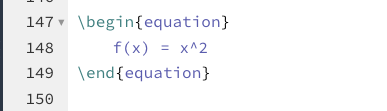
\includegraphics[scale=0.4]{equation.png}
    \caption{Creating an equation in a dedicated environment}
    \label{fig:equation}
\end{figure}  

Like for sections etc. you can omit the numbering by adding an asterisk, like this: \verb|\begin{equation*}|
\end{frame}

\begin{frame}[fragile]{Other expressions}
Fractions: $\frac{1}{x}$ is \verb|$\frac{1}{x}$|\\~\\
Integral: $\int^a_b \frac{1}{3}x^3$ is \verb|$\int^a_b \frac{1}{3}x^3$|\\~\\
Sum: $\sum_{i=1}^n$ is \verb|$\sum_{i=1}^n$|\\~\\
You can use as many of these expressions in one equation as you need. 
\end{frame}

\begin{frame}[fragile]{Aligning}
The amsmath package also allows you to align equations using the \textit{align} environment:\\
\begin{align*} 
2x - 5y &=  8 \\ 
3x + 9y &=  -12
\end{align*}
\begin{figure}
    \centering
    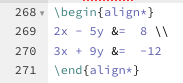
\includegraphics[width=0.3\textwidth]{align.png}
\end{figure}
\end{frame}

\begin{frame}{amsmath documentation}
Some helpful resources for writing equations:\\~\\
\begin{itemize}
    \item \href{https://mirror.foobar.to/CTAN/macros/latex/required/amsmath/amsldoc.pdf}{User's guide}
    \item \href{https://en.wikibooks.org/wiki/LaTeX/Mathematics}{Wikibooks LaTeX/Mathematics} 
    \item \href{https://latex-tutorial.com/tutorials/amsmath/}{Intro} with common expressions
    \item \href{https://www.overleaf.com/learn/latex/Aligning_equations_with_amsmath}{Overleaf tutorial}
\end{itemize}
\end{frame}

\begin{frame}[fragile]{Formulas}
\begin{figure}
    \centering
    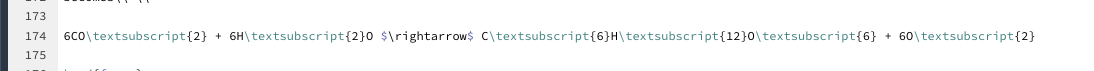
\includegraphics[width=\textwidth]{photosynth.png}
    \caption{}
    \label{fig:photosynth}
\end{figure}

becomes\\~\\

6CO\textsubscript{2} + 6H\textsubscript{2}O $\rightarrow$ C\textsubscript{6}H\textsubscript{12}O\textsubscript{6} + 6O\textsubscript{2}\\~\\
There is an easier way to write chemical equations, see frame \ref{frame:chem}.

\end{frame}

%-------------
\section{Bibliographies}
%------------

\begin{frame}{}
\LARGE \centering Bibliographies    
\end{frame}

\begin{frame}[fragile]{Creating a .bib file} 
In order to cite works and add a bibliography to the end of your document, you first need to add them to a \verb|.bib| file in the correct format.\\~\\
\pause
You can do this in Overleaf by creating a new file and naming it with the suffix \verb|.bib|, e.g. \verb|example.bib|.\\~\\
\pause
Alternatively, you can also create a .bib file using your text editor of choice, adding references and saving it as with the \verb|.bib| suffix or export them from reference managers like Zotero (more on that later).
\end{frame}

\begin{frame}[fragile]{Adding references}
References that are added to a LaTeX file need to be in a specific format.\\~\\
\pause
Luckily, sites like Google Scholar generally have the option of extracting a reference in the proper format; usually labelled as \textbf{BibTeX}.\\~\\
\pause
Then just copy and paste the reference and add it to your \verb|.bib| file, a.k.a. your bibliography.
\end{frame}

\begin{frame}{Adding references}
\begin{figure}
     \centering
     \begin{subfigure}[b]{0.45\textwidth}
         \centering
         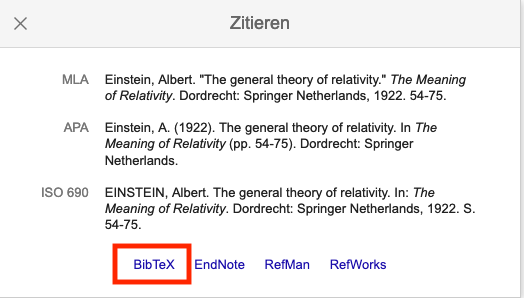
\includegraphics[width=\textwidth]{einstein_ref.png}
     \end{subfigure}
     \hfill
     \begin{subfigure}[b]{0.45\textwidth}
         \centering
         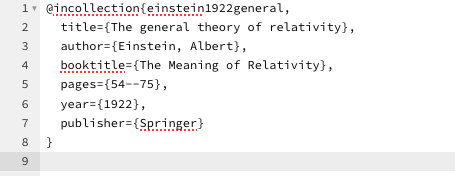
\includegraphics[width=\textwidth]{einstein_ref2.png}
     \end{subfigure}
     \caption{Access and copy-paste a BibTeX reference}
\end{figure}  
You can change the short name (here: \textit{einstein1922general}) to something else if you don't like the default.
\end{frame}

\begin{frame}[fragile]{Bibliography styles}
Using the standard BibTex format, you can cite works by using \verb|\cite{}| in text and choose a bibliography style, see \href{https://www.overleaf.com/learn/latex/Bibtex_bibliography_styles}{Bibtex bibliography styles}.\\~\\
Standard BibTex covers styles that use numbering or abbreviations inplace of full names for in-text citations.  
\end{frame}

\begin{frame}[fragile]{Bibliography styles}
In the following example, we use the \textbf{natbib} package to make the bibliography, a sort of add-on standard BibTex.\\~\\
\pause
To add the bibliography, put \verb|\bibliography{example}| at the end of the document (before \verb|\end{document}|)\\~\\
\pause
There are many different citation and bibliography styles, and each field has its own preferences. You can find an overview \href{https://www.overleaf.com/learn/latex/Bibtex_bibliography_styles}{here}.\\~\\
\pause
You can specify the style by adding e.g. \verb|\bibliographystyle{apalike}|, ideally after calling the natbib package.
\end{frame}

\begin{frame}[fragile]{Citing in text}
Using  the natbib package, you can cite works in your text by using \verb|\citet{}| and \verb|\citep{}|.\\~\\
\pause
Different disciplines have different citing standards, but generally, \verb|citet{}| is an ``ordinary" citation and \verb|\citep{}| puts the whole reference in parentheses.\\~\\
\pause
E.g. APA style: Einstein (1922) and (Einstein, 1922) respectively.\\~\\
\pause
\verb|\citep{}| can be used to cite multiple works.
\end{frame}

\begin{frame}[fragile]{Citing in footnotes}
\small You can either redefine the behaviour of your \texttt{\textbackslash cite} command or use a package like \textbf{jurabib} for specific citation behaviour in the Humanities.\\~\\
\pause
\texttt{\textbackslash jurabibsetup\\ \{authorformat=smallcaps,\\
commabeforerest,\\
ibidem=strict,\\
idem=strict,\\
titleformat={all,colonsep},	 {\color{green}\% cite always author and title}
\\
citefull=first,\\
lookforgender,\\
pages=always,\\
authorformat=firstnotreversed, {\color{green}\% Ed.: First name, surname}
\\
see, {\color{green}\%"Vgl."}
\\
super 	 {\color{green}\% always as footnote}\}}
\end{frame}

\begin{frame}[fragile]{Citing in footnotes}
You can also use bib styles developed by others or create one yourself (it's actually not that hard!) to change the behaviour of the default cite settings, using the package \textbf{biblatex}.\\~\\
\texttt{\textbackslash usepackage[backend=biber, style=mytry-footnote-dw,\\
edsuper=true,\\
editionstring=true,\\
edbyidem=true,\\
firstfull=false,\\
namefont=smallcaps,\\
\ldots\\
shorthandibid=true,\\
isbn=false]\{biblatex\}}
\end{frame}




\begin{frame}[fragile]{Multiple bibliographies}
In Humanities, you might need multiple bibliographies -- archival and printed sources, manuscript catalogues, research literature and whatnot. \\~\\
\pause
For this you can either use the package  \textbf{multibib} and define the different bibliographies using the command \texttt{\textbackslash newcites}, e.\ g.:\\~\\
\texttt{\textbackslash newcites\{prime,sec,third,fourth,fifth\}\{Quelleneditionen, Forschungsliteratur,Handschriften und ungedruckte Quellen,Inkunabeln und alte Drucke,Handschriftenkataloge\}}
\end{frame}

\begin{frame}[fragile]{Multiple bibliographies}
Or you can declare multiple bibliographies in the preambel:\\~\\
\texttt{\textbackslash DeclareBibliographyCategory\{sec\}}\\
\texttt{\textbackslash defbibheading\{sec\}\{\textbackslash section*\{Forschungsliteratur\}}\\
\texttt{\textbackslash newcommand*\{\textbackslash citesec\}[3]\{\textbackslash addtocategory\{sec\}\{#3\} \textbackslash cite[#1][#2]{#3}}
\end{frame}

\begin{frame}[fragile]{Multiple bibliographies}
Using the first option looks like this:\\~\\
\pause
\texttt{Here I am citing a source edition.\textbackslash citeprime[S. 230--498]\{hegel\_chroniken\_1870\}}\\~\\
\pause
In the document :\\
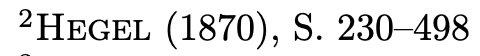
\includegraphics[scale=0.3]{footnote_citation.png}\\
\pause
At the end of the document in the bibliography:

\includegraphics[scale=0.2]{bibliography_citation.png}
\end{frame}

\begin{frame}[fragile]{Multiple bibliographies}
Using the second option looks like this:\\~\\
\pause
\texttt{Here I am citing research literature.\textbackslash footnote\{Zu mittelalterlichen Reiseberichten als Gattung \textbackslash citesec\{vgl.\}\{\}\{achnitz\_reiseberichte\_2012\}. \ldots}\}\\~\\
\pause
In the document :\\
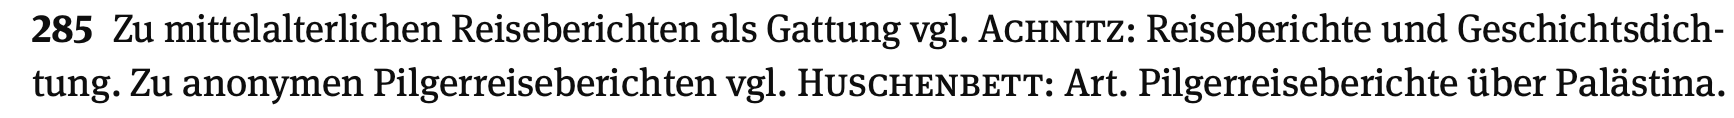
\includegraphics[scale=0.3]{footnote_citation_2.png}\\
\pause
At the end of the document in the bibliography:

\includegraphics[scale=0.3]{bibliography_citation_2.png}
\end{frame}




\begin{frame}{Resources}
\begin{itemize}
    \item \href{https://de.overleaf.com/learn/latex/Bibliography_management_in_LaTeX}{Bibliography management in LaTeX}
    \item \href{https://www.overleaf.com/learn/latex/Bibtex_bibliography_styles}{BibTeX bibliography styles}
    \item \href{https://www.overleaf.com/learn/latex/Bibliography_management_with_natbib}{Bibliography management with natbib}
    \item \href{https://de.overleaf.com/learn/latex/Natbib_citation_styles}{natbib citation styles}
    \item \href{https://www.ctan.org/pkg/jurabib}{Jurabib for law and humanities}
    \item \href{https://ctan.org/pkg/bibtex} {For citations in a document in the form specified by a BibTeX style} 
\end{itemize}    
\end{frame}

\begin{frame}{Integration with other bibliography software}
You can directly link your Overleaf account to Zotero or Mendeley - but that is a premium feature, unfortunately.\\~\\
Luckily, there are other ways of combining utilizing LaTeX in addition to other reference management software.\\~\\
\pause
The following example uses Zotero, but most reference managers should work along those same lines.
\end{frame}

\begin{frame}[fragile]{Zotero}
The easiest way to re-use your Zotero database is to \textbf{export} libraries to BibTeX format (i.e. a \verb|.bib| file)\\~\\
\pause
To do that, just go to \textit{File} $\rightarrow$ \textit{Export Library} to create a \verb|.bib| file that you can then upload to Overleaf or add to your LaTeX editor of choice.\\~\\
\pause
If you only want to export some but not all references, you can select them, then right click and choose \textit{Export...}
\end{frame}

\begin{frame}[fragile]{Chapter bibliographies}
I do not have personal experience with this, but there is a package called \textit{chapterbib} that allows you to put a select bibliography based on the same \verb|.bib| file after each chapter.\footnote{It's also possible to create different bibliographies for each chapter.}\\~\\
You can find a reproducible example \href{https://tex.stackexchange.com/questions/229846/different-bibliographies-for-each-chapter-with-shared-references}{here}.
\end{frame}

% others? citavi also has the function to export citations in bibtex format and has an integration with non-online editors
% maybe ask them what they're using

\begin{frame}[fragile]{Common Issues}
\begin{itemize}
    \item No capitalization: put curly brackets around either the capitalized letter or the whole word to make sure appears properly in the bibliography
    \item ? instead of reference in text: sometimes it takes a while to sync, so best option is to recompile; typo; missing info in reference
    \item Style suddenly changes: probably something off with the last reference you added to your \verb|.bib| file
\end{itemize}    
\end{frame}

%-------------
\section{Specialist packages}\label{spec_pack}
%------------

\begin{frame}{}
\LARGE \centering Specialist packages    
\end{frame}

\begin{frame}[fragile]{mhchem}\label{frame:chem}
\href{https://mirror.init7.net/ctan/macros/latex/contrib/mhchem/mhchem.pdf}{mhchem} offers a range of tools to write chemical expressions and reactions.\\~\\
\ce{CO2 + C -> 2 CO} and \ce{Sb2O3} can be written as \\~\\
\verb|\ce{CO2 + C -> 2 CO}| and \verb|\ce{Sb2O3}|
\end{frame}

\begin{frame}{Non-Latin alphabets}
Some languages do not require much extra work, and packages like \textit{fontenc} and \textit{inputenc} are enough, for example Greek.\\~\\
You can see an example \href{https://latex-ninja.com/2022/01/16/how-to-write-ancient-greek-in-latex/}{here}.
% Greek: fontenc, inputenc 
% https://latex-ninja.com/2022/01/16/how-to-write-ancient-greek-in-latex/
% also runes?
\end{frame}

\begin{frame}{Non-Latin alphabets}
Some languages may require you to change the \textit{compiler}. The standard is pdfLateX, but in Overleaf, you can easily change to XeLaTeX or LuaLaTeX.\\~\\
If you're working with multiple languages, it is recommended to additionally use the \textit{polyglossia} package.\\~\\
Generally, you can create dedicated sections/environments for most languages that also take \textit{direction} into account (left to right or vice versa)
\end{frame}

\begin{frame}{Non-Latin alphabets}

package \href{https://ctan.math.illinois.edu/fonts/allrunes/allrunes.pdf}{allrunes}
\begin{itemize}
    \item Germanic Runes: \textarc{fu\th \H j Rs M d}
    \item Anglo-Frisian Runes: \textara{fu\th \H j Rs M d}
    \item Normal Runes: \textarn{fu\th \H j Rs M d}
    \item Medieval Runes: \textarm{fu\th \H j Rs M d}
\end{itemize}
\end{frame}

\begin{frame}{Non-Latin alphabets}
Middle High/Low German(ic) characters
\pause
\begin{itemize}
    \item Superscripts, with \textbackslash usepackage[safe]\{tipa\} 
    \begin{itemize}
        \item z\r{u} mînem br\r{u}der\\
        \item r\sups{o}{e}msche k\"unge
    \end{itemize}
\pause
    \item Special characters:
    \begin{itemize}
        \item þÞ æ Æ ð Ð, with \textbackslash usepackage[icelandic]\{babel\} and \textbackslash usepackage[T1]\{fontenc\}
        \pause
        \item Use the \href{https://www.cl.uni-heidelberg.de/courses/ss19/wissschreib/material/symbols-a4.pdf}{symbols list} or the \textbf{xunicode} package (with another compiler, XeLaTeX).
    \end{itemize}
\end{itemize}
\end{frame}

\begin{frame}{Special fonts}
A lot of special fonts are available online -- you can even produce documents using \href{https://www.reddit.com/r/programming/comments/c9b7x/ever_wanted_to_use_comic_sans_in_your_latex/}{Comic Sans} (with a bit of passion and installation), or \textgoth{Gothic script}.
\end{frame}


\begin{frame}{Non-Latin alphabets}
Helpful resources:
\begin{itemize}
    \item \href{https://de.overleaf.com/learn/latex/Multilingual_typesetting_on_Overleaf_using_polyglossia_and_fontspec}{General overview} for multilingual typesetting \& polyglossia
    \item \href{https://junicode.sourceforge.io/}{Unicode reference list}
    \item \href{https://www.overleaf.com/learn/how-to/Changing_compiler}{Change the compiler}
    \item \href{https://www.overleaf.com/learn/latex/Chinese}{Chinese}: compiler change recommended
    \item \href{https://www.overleaf.com/learn/latex/Japanese}{Japanese}: \textit{CJKutf8} package, no compiler change needed
    \item \href{https://www.overleaf.com/learn/latex/Korean}{Korean}: compiler change required
\end{itemize}
\end{frame}

%-------------
\section{Self-help competencies}
%------------

\begin{frame}{Evaluation}
\begin{figure}
    \centering
    
\includegraphics[width=0.5\textwidth]{QRCode_Evaluation_LaTeX Crash Course.jpg}
    \caption{Scan the code or go here: \url{https://k11331.evasys.de/evasys/online.php?p=6L5LE}}
\end{figure}
\end{frame}

\begin{frame}{}
Google is your friend -- seriously!\\~\\
It's in no way bad to look for help online. StackOverflow and other forums are particularly useful for LaTeX questions.
\end{frame}

\begin{frame}{}
\begin{figure}
    \centering
    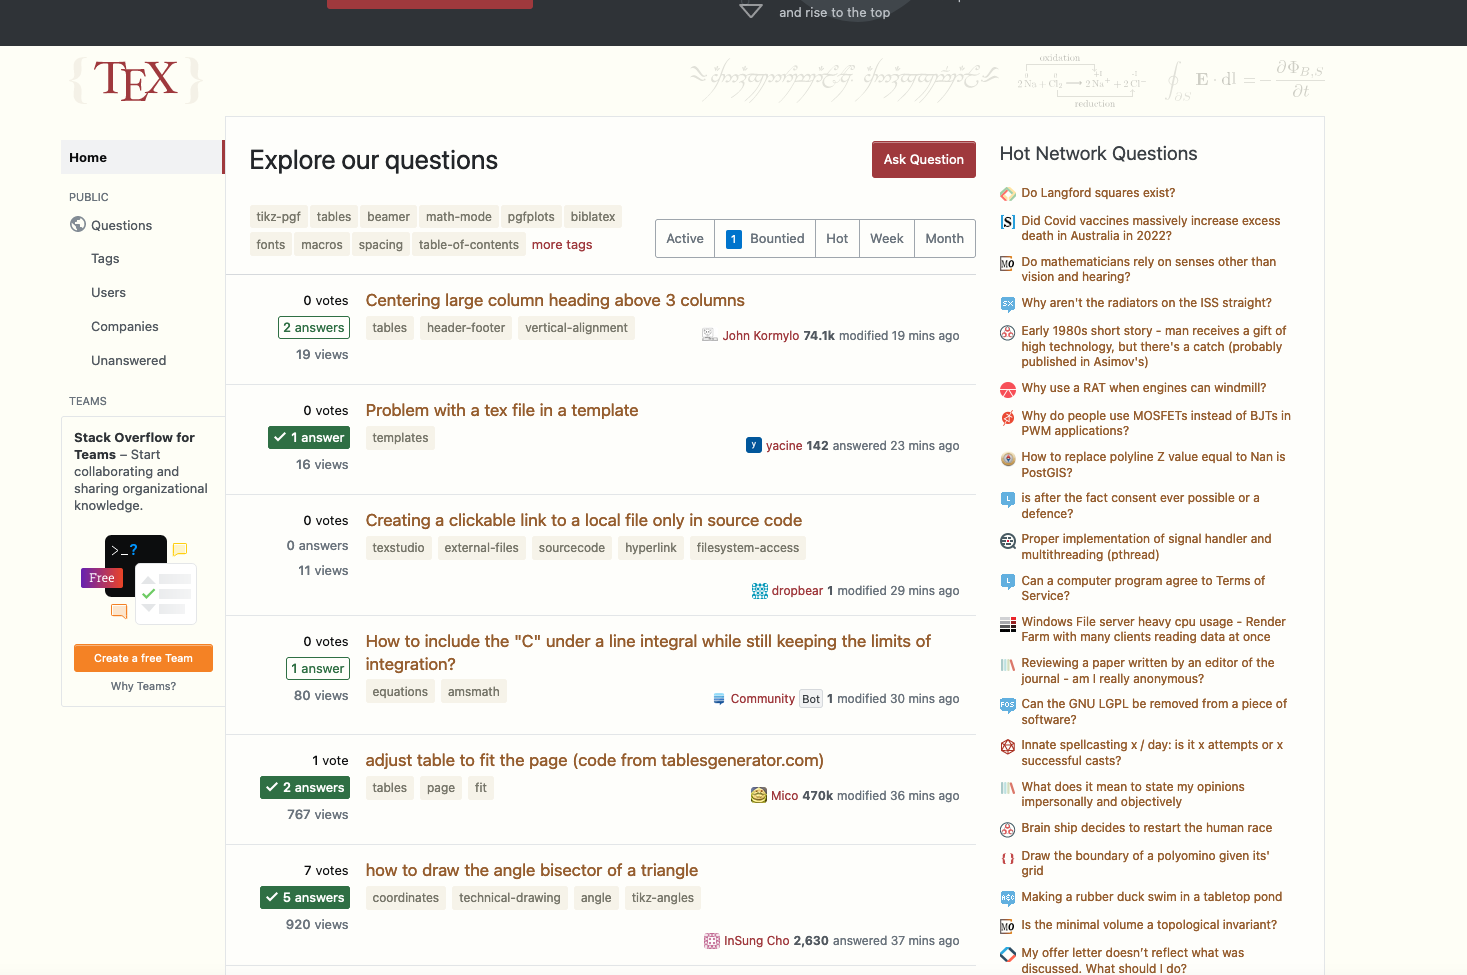
\includegraphics[width=0.7\textwidth]{tex_stack_overflow.png}
    \caption{Screenshot taken on March 29th 2023, 15:35}
    \label{fig:stack_overflow}
\end{figure}
\end{frame}

\begin{frame}{}
\begin{itemize}
    \item (Re-)Use templates -- your own or other people's (and materials from this course \smiley{})
    \item Overleaf has many \href{https://www.overleaf.com/latex/templates}{templates} and useful \href{https://www.overleaf.com/learn/latex/Tutorials}{tutorials}
    \item \href{https://en.wikibooks.org/wiki/LaTeX}{Wikibooks} on \LaTeX
    \item Practice, practice, practice
\end{itemize}    
\end{frame}


\end{document}
